\documentclass[11pt]{amsart}
\usepackage{hyperref}
\usepackage{amsmath,amssymb,amsfonts,amsthm,enumerate,natbib,color,ifthen}
\usepackage{xargs}
%\usepackage{calrsfs}
%\usepackage[notref,notcite]{showkeys}  %  comment out for final version
%\renewcommand*\showkeyslabelformat[1]{\fbox{\normalfont\scriptsize\sffamily#1}}   % for showkeys
\usepackage[textwidth=4cm, textsize=footnotesize]{todonotes}
\setlength{\marginparwidth}{4cm}    %  this goes with todonotes
\usepackage[latin1]{inputenc}



\usepackage{adjustbox}
\usepackage{multicol,booktabs,colortbl,tabularx}
\usepackage{caption,subcaption}
\usepackage{float}
%\usepackage[caption = false]{subfig}
\usepackage{graphicx}

\usepackage{aliascnt,bbm}
%\usepackage{algorithmicx}

%\usepackage{showlabels}
%\usepackage[latin1]{inputenc}
\renewcommand{\baselinestretch}{1.2}

%\topmargin -0.5cm
%\oddsidemargin -0.25cm
%\evensidemargin -0.25cm
%
%\textheight 9in
\textwidth 5.6in



% NOTATIONS
%%%%%%%%%%%%%
%%%%%%%%%%%%%
% Ensembles
\def\nset{{\mathbb{N}}}
\def\rset{\mathbb R}
\def\zset{\mathbb Z}
\def\qset{\mathbb Q}
\def\eqsp{\;}


\newcommand{\eg}{e.g.}
\newcommand{\ie}{i.e.}
\newcommand{\wrt}{with respect to}
\newcommand{\as}{\text{a.s.}}
\newcommand{\pscal}[2]{\left\langle#1,#2\right\rangle}

\newcommand{\un}{\ensuremath{\mathbbm{1}}}
\newcommand{\eqdef}{\ensuremath{\stackrel{\mathrm{def}}{=}}}
\newcommand{\eps}{\varepsilon}


\def\Eset{\mathsf{E}}
\def\Xset{\mathcal{Z}} % Espace d 'etat
\def\Zset{\mathcal{Z}} % Espace d 'etat
\def\Vset{\mathsf{V}} % Espace d 'etat
\def\Yset{\mathsf{Y}} % Espace d 'etat
\def\Xsigma{\mathcal{X}} % tribu sur X
\def\Tsigma{\mathcal{B}(\Theta)} % tribu sut Theta
\def\F{\mathcal{F}} % filtration
\def\B{\mathcal{B}} % filtration
\def\cB{\mathsf{B}} % filtration
\def\barB{\overline{B}} % filtration
\def\e{\mathcal{E}}
\def\dist{\textsf{d}}
\def\q{\mathsf{q}}
\def\E{\mathbb{E}}
\def\N{\mathcal{N}}
\def\M{\mathcal{M}}
\def\m{\mathsf{m}}
\def\Mt{\mathcal{M}_{2,\textsf{w}}^{(0)}}
\def\G{\mathcal{G}}
\def\D{\mathcal{D}}
\def\A{\mathcal{A}}
\def\bV{\mathcal{V}}
\def\cV{\check{\mathcal{V}}}
\def\H{\mathcal{H}}
\def\cov{\mathbb{C}\mbox{ov}}
\def\calK{\mathcal{K}}
\newcommandx\sequence[3][2=t,3=\zset]
{\ifthenelse{\equal{#3}{}}{\ensuremath{\{ #1_{#2}\}}}{\ensuremath{\{ #1_{#2}, \eqsp #2 \in #3 \}}}}

%\DeclareMathAlphabet{\pazocal}{OMS}{zplm}{m}{n}
\newcommand{\Sa}{\mathcal{S}}
%\newcommand{\Sb}{\pazocal{S}}




\def\PP{\mathbb{P}} % proba
\newcommand{\CPP}[3][]
{\ifthenelse{\equal{#1}{}}{{\mathbb P}\left(\left. #2 \, \right| #3 \right)}{{\mathbb P}_{#1}\left(\left. #2 \, \right | #3 \right)}}
\def\PE{\mathbb{E}} % esperance
\newcommand{\CPE}[3][]
{\ifthenelse{\equal{#1}{}}{{\mathbb E}\left[\left. #2 \, \right| #3 \right]}{{\mathbb E}_{#1}\left[\left. #2 \, \right | #3 \right]}}

\def\bPP{\overline{\mathbb{P}}} % proba sur espace double
\def\bPE{\overline{\mathbb{E}}} % esperance sur espace double
\def\cPP{\check{\mathbb{P}}} % proba sur espace quadruple
\def\cPE{\check{\mathbb{E}}} % esperance sur espace quadruple
\def\cP{\check{P}} % proba
\def\wtilde{\widetilde} % proba



\def\lyap{\omega}
\def\W{\mathcal{W}}
\def\K{\mathcal{K}}
\def\L{\mathcal{L}} % espace des fonctions
\def\Vs{V_\star}
\def\V{\mathbb{V}}
\def\ns{n_\star}
\def\tv{\mathrm{tv}}
\def\tvs{\mathrm{tv(s)}}
\def\tauout{\stackrel{\leftarrow}{\tau}} % temps de sortie
\def\compact{\mathsf{K}}  % compact
\def\Cset{\mathcal{C}} % Petite set
\def\Dset{\mathcal{D}} % Generic set
\newcommand{\dlim}{\ensuremath{\stackrel{\mathcal{D}}{\longrightarrow}}}
\newcommand{\plim}[1]{\ensuremath{\stackrel{\mathrm{P}_{#1}}{\longrightarrow}}}
\newcommand{\aslim}{\ensuremath{\stackrel{\text{a.s.}}{\longrightarrow}}}
\newcommand\Plim[1]{\mathbb{Q}_{#1}}
\newcommand{\abs}[1]{\left\vert#1\right\vert}
\newcommand{\norm}[1]{\left\Vert#1\right\Vert}
\newcommand{\normoff}[1]{\left\Vert#1\right\Vert_{1,\textsf{off}}}
\newcommand{\normfro}[1]{\left\Vert#1\right\Vert_{\textsf{F}}}

\newcommand{\tnorm}[1]{\left\vert\!\left\vert\!\left\vert#1\right\vert\!\right\vert\!\right\vert}
\newcommand{\nnorm}[1]{\left\Vert#1\right\Vert_2}
\newcommand{\inte}[1]{\stackrel{\circ}{#1}}


\def\Rg{\mathsf{Rg}}
\def\barlambda{\underline{\Lambda}}
\def\Mb{\mathcal{M}_\textsf{b}}
\def\b{\textsf{b}}
\def\piq{\textsf{q}}
\def\I{\textsf{I}}
\def\t{\textsf{T}}
\def\w{\textsf{w}}
\def\c{\textsf{c}}
\def\sp{\textsf{sp}}
\def\deg{\textsf{deg}}
\def\Prox{\operatorname{Prox}}
\def\Proxj{\textsf{Prox}^{[j]}}
\def \thetagl{\hat\theta_{\textsf{gl}}}
\def \thetalasso{\hat\theta_{\textsf{lasso}}}
\def\vec{\textsf{Vec}}
\def\mat{\textsf{Mat}}
\def\r{\textsf{r}}


\usepackage{bm}%bold matH
\def\bzero{{\bf 0}}







% DIALOGUES ENTRE AUTEURS
%%%%%%%%%%%%%%%%%%%%%%%%%
%\newcommand{\comment}[2]{\begin{quote}\color{#1}\begin{sffamily} #2 \end{sffamily}\color{black}\end{quote}}
%\newcommand{\note}[2]{\marginpar{\parbox[t]{\noteWidth}{\raggedright\textcolor{blue}{\tiny{#2}} \textcolor{red}{\tiny{#1}}}}}
%
%\def\yves{blue}
%\def\eric{red}
%\newlength{\noteWidth}
%\setlength{\noteWidth}{.6in}
%\newcommand{\yves}[1]{\todo[color=green!20]{{\bf Y:} #1}}
%\newcommand{\anwesha}[1]{\todo[color=blue!20]{{\bf A:} #1}}




\theoremstyle{plain}
\newtheorem{theorem}{Theorem}
\newtheorem{assumption}{H\hspace{-3pt}}
\newtheorem{assumptionB}{B\hspace{-3pt}}
\newtheorem{assumptionC}{C\hspace{-3pt}}
\newtheorem{problem}{P}


\newaliascnt{proposition}{theorem}
\newtheorem{proposition}[proposition]{Proposition}
\aliascntresetthe{proposition}

\newaliascnt{lemma}{theorem}
\newtheorem{lemma}[lemma]{Lemma}
\aliascntresetthe{lemma}
\newaliascnt{corollary}{theorem}
\newtheorem{corollary}[corollary]{Corollary}
\aliascntresetthe{corollary}


 \newtheorem{conjecture}{Conjecture}[section]
\newtheorem{hypothese}{Hypothesis}
\newtheorem{fact}[theorem]{Fact}


\theoremstyle{definition}
\newaliascnt{definition}{theorem}
\newtheorem{definition}[definition]{Definition}
\aliascntresetthe{definition}

%\newaliascnt{algorithm}{theorem}             % uncomment these 3 lines and comment line 90 if dont want float
%\newtheorem{algorithm}[algorithm]{Algorithm}
%\aliascntresetthe{algorithm}
\newtheorem{algorithm}{Algorithm}

\newaliascnt{remark}{theorem}
\newtheorem{remark}[remark]{Remark}
\aliascntresetthe{remark}

\newaliascnt{example}{theorem}
\newtheorem{example}[example]{Example}
\aliascntresetthe{example}



\providecommand*{\definitionautorefname}{Definition}
\providecommand*{\lemmaautorefname}{Lemma}
\renewcommand*{\subsectionautorefname}{Section}
\renewcommand*{\subsubsectionautorefname}{Section}
\providecommand*{\exampleautorefname}{Example}
\providecommand*{\propositionautorefname}{Proposition}
\providecommand*{\procautorefname}{Procedure}
\providecommand*{\exerciseautorefname}{Exercise}
\providecommand*{\corollaryautorefname}{Corollary}
\providecommand*{\remarkautorefname}{Remark}
\providecommand*{\algorithmautorefname}{Algorithm}

\providecommand*{\assumptionautorefname}{H\hspace*{-2.5pt}}  %hspace is stretchable, but \! is not and \!\! is too much
\providecommand*{\problemautorefname}{(P)\hspace*{-2.5pt}}  %hspace is stretchable, but \! is not and \!\! is too much


\newcommand{\coint}[1]{\left[#1\right)}
\newcommand{\ocint}[1]{\left(#1\right]}
\newcommand{\ooint}[1]{\left(#1\right)}
\newcommand{\ccint}[1]{\left[#1\right]}

\def\rmd{\mathrm{d}}
\def\rme{\mathrm{e}}
\def\PG{\operatorname{PG}}
\def\1{\mathbbm{1}}
\def\gauss{\operatorname{N}}
\def\bU{\mathbf{U}}
\def\bY{\mathbf{Y}}
\def\bu{\mathbf{u}}
\def\bW{\mathbf{W}}
\def\bw{\mathbf{w}}
\def\stdnor{\mathbf{N}}
\def\iid{i.i.d.}
\newcommand{\ball}[2]{\mathcal{B}(#1,#2)} 


%From Rahul
\newcommand{\sbt}{\mbox{subject to}}
\DeclareMathOperator*{\mini}{minimize}
\DeclareMathOperator*{\maxi}{maximize}
%\def\argmin{\operatorname{Argmin}}
\DeclareMathOperator*{\argmin}{{\textsf{Argmin}}}






\def\code#1{\texttt{#1}}
\newcommand{\RomanNumeralCaps}[1]
    {\MakeUppercase{\romannumeral #1}}
\usepackage{hyperref}
\usepackage{caption,subcaption} 
\usepackage{tikz,pifont}
\usepackage{amssymb,mathtools,amsmath}
\usepackage[nameinlink,noabbrev]{cleveref}
\usepackage{natbib}

\setlength{\textwidth}{\paperwidth}
\addtolength{\textwidth}{-1.5in}
\calclayout

\hypersetup{
    colorlinks=true,
    linkcolor=red,
    filecolor=red,      
    urlcolor=red,
    citecolor=blue,
    linktoc=page
}

\makeatletter
\def\@tocline#1#2#3#4#5#6#7{\relax
  \ifnum #1>\c@tocdepth % then omit
  \else
    \par \addpenalty\@secpenalty\addvspace{#2}%
    \begingroup \hyphenpenalty\@M
    \@ifempty{#4}{%
      \@tempdima\csname r@tocindent\number#1\endcsname\relax
    }{%
      \@tempdima#4\relax
    }%
    \parindent\z@ \leftskip#3\relax \advance\leftskip\@tempdima\relax
    \rightskip\@pnumwidth plus4em \parfillskip-\@pnumwidth
    #5\leavevmode\hskip-\@tempdima
      \ifcase #1
       \or\or \hskip 1em \or \hskip 2em \else \hskip 3em \fi%
      #6\nobreak\relax
    \hfill\hbox to\@pnumwidth{\@tocpagenum{#7}}\par% <---- \dotfill -> \hfill
    \nobreak
    \endgroup
  \fi}
\makeatother

\setcounter{tocdepth}{5}
\setcounter{secnumdepth}{5}
\begin{document}

\title[Aging]{ Title \\ \today }


\keywords{Aging}

\maketitle
\begin{abstract}
	 
\end{abstract} 

\tableofcontents

\newpage

\section{Introduction}

On average, mortality rates in humans tend to increase exponentially with age. However, this mortality rate does not apply uniformly to all humans in an age group; there is an observed heterogeneity in mortality and health status among individuals in an age cohort. One 80-year-old may have a long list of health issues, limited mobility, and cognitive deficits, while another may seem a decade younger than their true age. The difference in the rate of aging between individuals creates a difference between chronological and biological age. The concept of frailty is used to capture this phenomenon.
 
Frailty is defined in the literature as the state of increased vulnerability to adverse health outcomes. Identifying frailty is an important clinical challenge as frail individuals tend to have both increased risk of diseases and disorders, worse health outcomes from the same disease, and even different symptoms of the same disease \citep{whitehead2014clinical}. Their all-cause mortality risk is also higher than non-frail individuals of a similar age.
 
Though how to best quantify frailty is still controversial, one popular method is to use a frailty index (FI). In this method, an individual is scored on a set of age-related deficits as either 0 (no deficit), 0.5 (slight deficit), or 1 (deficit present). The scores are added up and divided by the total number of deficits in the frailty index, giving a final FI score. Studies have shown that the specific items included in a FI, provided they meet certain criteria, are not important \citep{rockwood2017frailty}. The criteria for items to be included in a FI are: 1) that the deficits are health-related; 2) that the deficits generally increase with age; 3) that the FI is composed of more than 30 different items; and 4) that the items in the FI do not saturate (e.g. become apparent in all individuals) at too early an age \citep{searle2008standard}. Frailty indexes constructed which fulfill the above requirements have consistent characteristics shared between them: average FI scores increase exponentially with age, variability in FI scores also increases with age, the score strongly predicts risk of adverse outcomes and mortality, and there is a submaximal limit of about $\frac{2}{3}$ of deficits accumulated after which the individual dies \citep{searle2008standard}. Although human frailty indexes have been studied extensively, it is only recently that researchers have recreated one for mice. 
 
In mice, the frailty index consists of 30 set features which can be graded without the use of specialized equipment. In a 2017 study by \citet{rockwood2017frailty} comparing the mouse frailty index across lifespan of two hundred fifty-one male C57BL/6J to human FI data, the mouse CFI showed several essential features seen with human aging. The mouse CFI had a similar distribution to humans where the mean FI score increased exponentially with age with comparable values at comparable life stages. The FI scores also showed a dose-response relationship with mortality and a submaximal limit. Although individual deficit accumulation patterns varied, the distribution of the frailty index broadened with age and mean deficit accumulation increased. At all ages, greater deficit accumulation was associated with reduced survival in age-adjusted models. These results point to the potential usefulness of the FI concept for a preclinical model of frailty and aging. Indeed, the mouse CFI has since been used to evaluate interventions on frailty such as administering resveratrol and caloric restrictions, and to study the changes in aging of the microbiome, inflammation, genetics, and heart health \citep{kane2017implementation}.

Unlike the human frailty index, most mouse frailty indexing has been done with the same set of 30 features. It is likely though, that just as the human frailty index is robust to different sets of deficits, a new mouse CFI can be constructed. Indeed, some studies have already substituted a small number of mouse CFI features for ones that fit their specific strain or experiment \citep{kane2017implementation}. We propose that we can use this characteristic of frailty indexes to construct our own. We hypothesize that biological aging produces changes in behavior and physiology which can be captured with our video assay. Our goal is to develop an efficient and scalable visual frailty index from video metrics using modeling. Such an FI could be used to study mechanisms, exacerbators, and interventions for biological aging on a large scale. 

\section{Methods}
Two hundred fifty-three C57BL/6J mice of varying ages were put in the one-hour open field test with top-down video taken. They were then given a frailty index score by trained scorers. The ages of the mice ranged from 20 to 134 weeks. There were 161 males and 92 females. Below is a plot showing CFI scores by age, colored for sex (males in blue, females in red):

\begin{center}

Leinani's figure

\end{center} 




Though the overall trend for the mean is to increase with age group, there is a slight dip between 80 to 100 weeks. Further, although standard deviation of the group increased with age group, after 40 weeks the increase is only slight.

In order to see how the scorer had an effect on ratings, a plot graphing FI by age colored by the scorer was made:

\begin{center}

Leinani's figure

\end{center} 


The plot reveals some obvious scorer effects. The red scorer tended to have slightly higher CFI scores while the purple scorer tended to have slightly lower CFI scores. In the 70 to 90 week age range, the turquoise scorer was dominant, combined with the purple scorer, and they tended towards lower CFI scores. This may explain the slight dip seen in group means.

The videos of each mouse were run through our open field pipeline which consists of the standard gait metrics and the open field metrics. For a review of these metrics refer to (*********)

In addition to our standard pipeline features, we engineered features from the video data. The first feature we looked at was flexibility. Spinal mobility in humans is a predictor for quality of life in aged populations \citep{imagama2011back} and the mouse is used as a model for the aging human spine (Holguin et al., 2014). Thus, we hypothesized that aged mice may bend their spine to a lesser degree, or less often due to reduced flexibility or spine degeneration. This change in flexibility can be captured by the pose estimation. In this approach, we take the coordinates of three points on the mouse at each video frame: the back of the head (A), the middle of the back (B), and the base of the tail (C). A line is drawn through the points. Tracking the length of the line AC normalized for mouse length (dAC), the orthogonal distance of the middle of the back B from the line (dB), and the angle of the three points (aABC) is used as a measure of the bend in the spine. For each of the three per frame measures (dAC, dB, and aABC) a mean, median, standard deviation, minimum, and maximum are calculated per video. These become the features to be used in the model.

\begin{center} 

Leinani's figure

\end{center} 

The next engineered features were body composition features. In humans, anthropometric measures such as BMI and waist-to-hip ratio are predictors for certain health conditions and mortality risk. Aging is associated with changes in body composition, increased visceral fat and decreased subcutaneous fat, progressive dysfunction of adipose tissue, and changes in ratio of brown and white adipose tissue \citep{huffman2009role}. These changes are also seen in obese patients, making them present as prematurely aged.  Though obesity, as defined by BMI, is a predictor for various metabolic disorders, cardiovascular disorders, cognitive disorders, and overall mortality risk, it seems that visceral fat is a strong causal factor \citep{huffman2009role}. Visceral fat creates a systemic inflammatory environment via secretion of inflammasomes. This ties visceral fat to the popular theory of aging: ``Inflammaging'', where aging is caused or exacerbated by chronic low grade inflammation \citep{perez2016adipaging}. Visceral fat is a better predictor for various health issues and mortality than BMI \citep{scafoglieri2014use}. This is thought to be because BMI can sometimes be a poor predictor of visceral fat. Further, anthropometric measures tend to vary based on measurement points and are also unreliable measures of visceral fat, though they may still be good predictors of risk of disorders and mortality. 

In mice, changes in body composition are observed as well \citep{pappas2019translation}. So far, no body measurements have been shown to solidly predict visceral fat, and specialized equipment must be used to predict fat composition. We observed that body weight was very highly correlated with the gait metrics with the highest correlations with FI score. Thus, we hypothesize that body composition metrics may show some signal for aging and frailty. On each frame, an ellipse was fitted to the mouse, giving a width and a length. The means and medians of the mouse width were used as features. Further, we took the coordinates of the rear paws of the mice per frame as a estimation of hip width. The mean and median rear paw width were also used as features for the model.

  We also looked into features related to intra-mouse variability of gait. A known part of aging is the heterogeneity in the presence of aging related metrics across an age group--heterogeneity in the age group increases with age group. This is a characteristic of the frailty index. There is also interest in heterogeneity at the individual level. In addition to looking at inter-group heterogeneity in gait, we looked at intramouse heterogeneity in gait using standard deviation and interquartile range of the mouse for each gait metric. The standard deviations and interquartile ranges were used as features for the model.






\section{ML}
Our goal is to predict age and frailty index (FI) from video data (gait phenotypes, open field metrics, engineered features) as accurately as possible. There are several different sets of video features that include animal features, gait features, open field metrics and engineered features available for modeling age and FI. 

We fit models in Table \ref{models} using a variety of machine learning methods. We use repeated 10-fold cross-validation with 10 repeats to assess the performance of our machine learning methods. 


Before buidling the models, we will split the data into training and test sets. The training set will be used to explore features, tune hyper-parameters, develop and compare models (\ref{models}). The test set will be used to arrive at a final, unbiased assessment models' performance. To partition the data, we split the original data (n = 252) in a {\textit{stratified}} manner to preserve the class distribution of the score. This will keep the distribution of animal scores approximately the same (\Cref{figure1}). 

\begin{figure}[h]
\centering
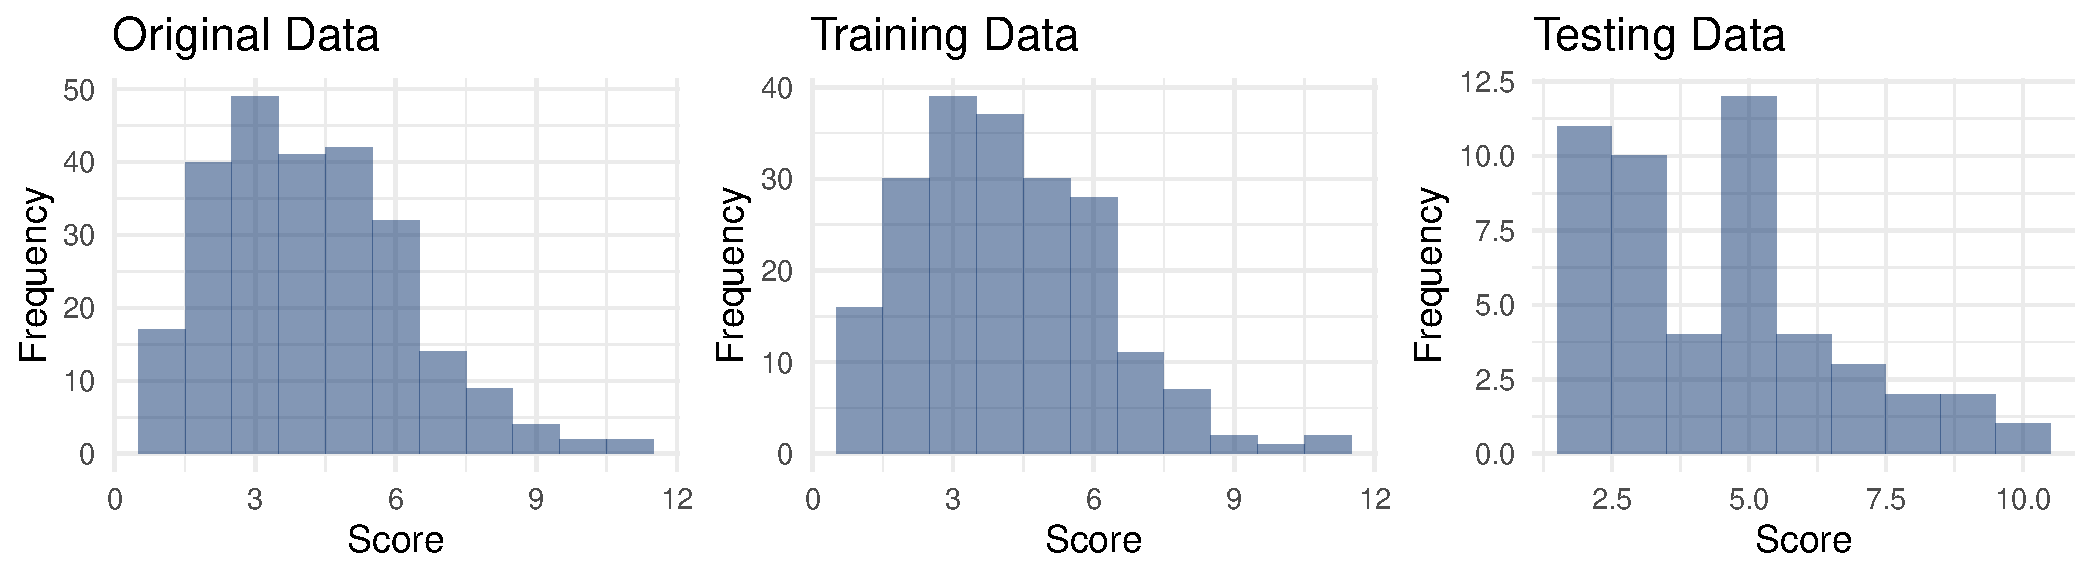
\includegraphics[width=150mm]{TeXPlots/figure1.pdf}
\caption{Distribution of scores}
\label{figure1}
\end{figure}

\begin{table}[h]
\centering
\begin{tabular}{|c|c|c|}
\hline
Model & Input & Output \\ 
\hline
M1 & Frailty features & Age \\
\hline 
M2 & Video features & Age \\
\hline 
M3 & Video features & FI \\
\hline 
M4 & Age & FI \\
\hline
\end{tabular}
\caption{We compare the performance of video features in predicting age (M2) with frailty parameters in predicting age (M1). Similarly we compare performace of video features with age in predicting FI (M3 vs M4).}
\label{models}
\end{table}

Our modeling process proceeds as follows,
\begin{itemize} 
  \item Pre-processing the input features.
  \item E


\newpage
\bibliographystyle{ims}
\bibliography{references}
\end{document}